\section{Disentangling Adversarial Robustness\\[2px]\hspace*{-6px}and Generalization}
\label{sec:main}

To clarify the relationship between adversarial robustness and generalization, we explicitly distinguish between regular and on-manifold adversarial examples, as illustrated in \figref{fig:introduction}. Then, the hypothesis \cite{TsiprasARXIV2018,SuARXV2018} that robustness and generalization are contradicting goals is challenged in four arguments: regular \red{unconstrained} adversarial examples leave the manifold; adversarial examples constrained to the manifold exist; robustness against on-manifold adversarial examples is essentially generalization; \red{robustness against regular adversarial examples is not influenced by generalization when controlled through the amount of training data}. Altogether, our results imply that adversarial robustness and generalization are not opposing objectives \red{and both robust and accurate models are possible} but require higher sample complexity.

\vskip 0px
\subsection{Experimental Setup}

\myparagraph{Datasets:} We use \MNIST \cite{CohenARXIV2017}, F(ashion)-MNIST \cite{XiaoARXIV2017} and \Celeb \cite{LiuICCV2015} for our experiments ($240\text{k}/40\text{k}$, $60\text{k}/10\text{k}$ and $182\text{k}/20\text{k}$ training/test images); \Celeb has been re-sized to $56{\times}48$ and we classify ``Male'' \vs ``Female''. Our synthetic dataset, \Fonts, consists of letters ``A'' to ``J'' of $1000$ Google Fonts randomly transformed (uniformly over translation, shear, scale, rotation in $[-0.2,0.2]$, $[-0.5,0.5]$, $[0.75,1.15]$, $[-\nicefrac{\pi}{2},\nicefrac{\pi}{2}]$) using a spatial transformer network \cite{JaderbergNIPS2015} such that the generation process is completely differentiable. The latent variables correspond to the transformation parameters, font and class. We generated $960\text{k}/40\text{k}$ (balanced) training/test images of size $28{\times}28$.

We consider classifiers with three (four on \Celeb) convolutional layers ($4\times4$ kernels; stride $2$; $16$, $32$, $64$ channels), each followed by ReLU activations and batch normalization \cite{IoffeICML2015}, and two fully connected layers. The networks are trained using ADAM \cite{KingmaICLR2015}, with learning rate $0.01$ (decayed by $0.95$ per epoch), weight decay $0.0001$ and batch size $100$, for $20$ epochs. Most importantly, to control their generalization performance, we use $N$ training images, with $N$ between $250$ and $40\text{k}$; for each $N$, we train $5$ models with random weight initialization \cite{GlorotAISTATS2010} an report averages.

We learn class-specific \VAEGANs, similar to \cite{LarsenICML2016,RoscaARXIV2017}, to approximate the underlying manifold; we refer to the supplementary material for details.

\myparagraph{Attack:} Given an image-label pair $(x,y)$ from an unknown data distribution $p$ and a classifier $f$, an adversarial example is a perturbed image $\tilde{x} = x + \delta$ which is mis-classified by the model, \ie, $f(\tilde{x}) \neq y$. While our results can be confirmed using other attacks and norms (see the supplementary material for \cite{CarliniSP2017} and transfer attacks), for clarity, we concentrate on the $L_{\infty}$ white-box attack by Madry \etal \cite{MadryICLR2018} that directly maximizes the training loss,
\vskip -14px
\begin{align}
	\max_\delta \cL(f(x + \delta), y)\quad\text{s.t.}\quad\|\delta\|_{\infty} \leq \epsilon, \tilde{x}_i \in [0,1],\label{eq:main-off-manifold-attack}
\end{align}
\vskip -2px
\noindent using projected gradient descent; where $\cL$ is the cross-entropy loss and $\tilde{x}=x+\delta$. The $\epsilon$-constraint is meant to ensure perceptual similarity. We run $40$ iterations of ADAM \cite{KingmaICLR2015} with learning rate $0.005$ and consider $5$ restarts, (distance and direction) uniformly sampled in the $\epsilon$-ball for $\epsilon = 0.3$. Optimization is stopped as soon as the predicted label changes, \ie, $f(\tilde{x}) \neq y$. We attack $1000$ test images.

\begin{figure}
    \centering
    \vskip -0.3cm
    \hskip -0.1cm
    \begin{subfigure}[t]{0.5\textwidth}
        \begin{subfigure}[t]{0.49\textwidth}
            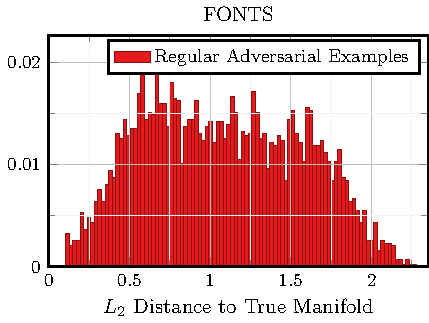
\includegraphics[width=0.9\textwidth]{experiments_hypo1_b.pdf}
        \end{subfigure}
        \begin{subfigure}[t]{0.49\textwidth}
            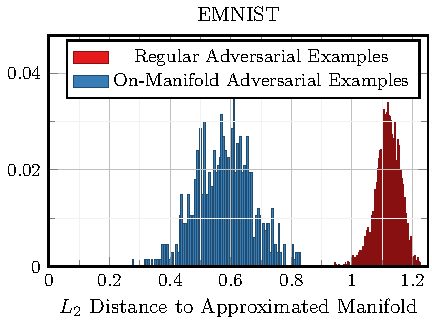
\includegraphics[width=0.9\textwidth]{experiments_hypo1_c.pdf}
        \end{subfigure}
    \end{subfigure}
    \vskip -6px
    \caption{Distance of adversarial examples to the true, on \Fonts (left), or approximated, on \MNIST (right), manifold. We show normalized histograms of the $L_2$ distance of adversarial examples to their projections onto the manifold ($4377$/$3837$ regular adversarial examples on \Fonts/\MNIST; $667$ on-manifold adversarial examples on \MNIST). Regular adversarial examples exhibit a significant distance to the manifold; on \MNIST, clearly distinguishable from on-manifold adversarial examples.}
    \label{fig:main-hypo1}
    \vskip 0px
\end{figure}

\myparagraph{Adversarial Training:} An established defense is adversarial training, \ie, training on adversarial examples crafted during training \cite{ZantedschiAISEC2017,MiyatoICLR2016,HuangARXIV2015,ShahamNEUROCOMPUTING2018,SinhaICLR2018,LeeARXIV2017b,MadryICLR2018}. Madry \etal \cite{MadryICLR2018} consider the min-max problem
\vskip -14px
\begin{align}
	\hskip -8px \min_w \sum_{n = 1}^N{\max_{\|\delta\|_{\infty} \leq \epsilon,x_{n,i}{+}\delta_i\in[0,1]}}{\cL}(f(x_n{+}\delta; w), y_n)
	\label{eq:main-off-manifold-adversarial-training}
\end{align}
\vskip -2px
\noindent where $w$ are the classifier's weights and $x_n$ the training images. As shown in the supplementary material, we considered different variants \cite{SzegedyARXIV2013,GoodfellowARXIV2014,MadryICLR2018}; in the paper, however, we follow common practice and train on $50\%$ clean images and $50\%$ adversarial examples \cite{SzegedyARXIV2013}. For $\epsilon = 0.3$, the attack (for the inner optimization problem) is run for full $40$ iterations, \ie, is not stopped at the first adversarial example found. Robustness of the obtained network is measured by computing the attack \textbf{success rate}, \ie, the fraction of successful attacks on correctly classified test images, as, \eg, in \cite{CarliniSP2017}, for a fixed~$\epsilon$; lower success rate indicates higher robustness of the network.

\vskip 0px
\subsection{Adversarial Examples Leave the Manifold}

The idea of adversarial examples leaving the manifold is intuitive on \MNIST where particular background pixels are known to be constant, see \figref{fig:main-examples}. If an adversarial example $\tilde{x}$ manipulates these pixels, it has zero probability under the data distribution and its distance to the manifold, \ie, the distance to its projection $\pi(\tilde{x})$ onto the manifold, should be non-zero. On \Fonts, with known generative process in the form of a decoder $\dec$ mapping latent variables $z$ to images $x$, the projection is obtained iteratively: $\pi(\tilde{x}) = \dec(\tilde{z})$ with $\tilde{z} = \argmin_{z} \|\dec(z) - \tilde{x})\|_2$ and $z$ constrained to valid transformations (font and class, known from the test image $x$, stay constant). On \MNIST, as illustrated in \red{\figref{fig:main-illustration-2} (right)}, the manifold is approximated using $50$ nearest neighbors; the projection $\pi(\tilde{x})$ onto the sub-space spanned by the $x$-centered nearest neighbors is computed through least squares. On both \Fonts and \MNIST, the distance $\|\tilde{x} - \pi(\tilde{x})\|_2$ is considered to asses whether the adversarial example $\tilde{x}$ actually left the manifold.

On \Fonts, \figref{fig:main-hypo1} (left) shows that regular adversarial examples clearly exhibit non-zero distance to the manifold. In fact, the projections of these adversarial examples to the manifold are almost always the original test images; as a result, the distance to the manifold is essentially the norm of the corresponding perturbation: $\|\tilde{x} - \pi(\tilde{x})\|_2 \approx \|\tilde{x} - x\|_2 = \|\delta\|_2$. This suggests that the adversarial examples leave the manifold in an almost orthogonal direction. On \MNIST, in \figref{fig:main-hypo1} (right), these results can be confirmed in spite of the crude local approximation of the manifold. Again, regular adversarial examples seem to leave the manifold almost orthogonally, \ie, their distance to the manifold coincides with the norm of the corresponding perturbations. These results show that regular adversarial examples essentially \emph{are} off-manifold adversarial examples; this finding is intuitive as for well-trained classifiers, leaving the manifold should be the ``easiest'' way to fool it; \red{results on \Fashion as well as a more formal statement of this intuition can be found in the supplementary material.}

\vskip 0px
\subsection{On-Manifold Adversarial Examples}

Given that regular adversarial examples leave the manifold, we intend to explicitly compute on-manifold adversarial examples. To this end, we assume our data distribution $p(x,y)$ to be conditional on the latent variables $z$, \ie, $p(x,y|z)$, corresponding to the underlying, low-dimensional manifold. \red{On this manifold, however, there is no notion of ``perceptual similarity'' in order to ensure label invariance, \ie, distinguish valid on-manifold adversarial examples, \figref{fig:introduction} (b), from invalid ones that change the actual, true label, \figref{fig:introduction} (c):}

\begin{definition}[On-Manifold Adversarial Example]
    Given the data distribution $p$, an on-manifold adversarial example for $x$ with label $y$ is a perturbed version $\tilde{x}$ such that $f(\tilde{x}) \neq y$ but $p(y | \tilde{x}) > p(y' | \tilde{x}) \forall y' \neq y$.\label{def:main-on-manifold-adversarial-example}
\end{definition}
\vskip 2px

\noindent Note that the posteriors $p(y|\tilde{x})$ correspond to the true, unknown data distribution; any on-manifold adversarial example $\tilde{x}$ violating \defref{def:main-on-manifold-adversarial-example} changed its actual, true label.

In practice, we assume access to an encoder and decoder modeling the (class-conditional) distributions $p(z|x,y)$ and $p(x|z,y)$ -- in our case, achieved using \VAEGANs \cite{LarsenICML2016,RoscaARXIV2017}. Then, given the encoder \red{$\enc$ and decoder $\dec$} and as illustrated in \figref{fig:main-illustration-2} (left), we obtain the latent code $z = \enc(x)$ and compute the perturbation $\zeta$ by maximizing:
\vskip -14px
\begin{align}
\max_\zeta \cL(f(\dec(z + \zeta)), y)\quad\text{s.t.}\quad\|\zeta\|_{\infty}\leq \eta.\label{eq:main-on-manifold-attack}
\end{align}
\vskip -2px
\noindent The image-constraint, \ie, $\dec(z + \zeta) \in[0,1]$, is enforced by the decoder; the $\eta$-constraint can, again, be enforced by projection; and we can additionally enforce a constraint on $z + \zeta$, \eg, corresponding to a prior on $z$. Label invariance, as in \defref{def:main-on-manifold-adversarial-example}, is ensured by considering only class-specific encoders and decoders, \ie, the data distribution is approximated per class. We use $\eta = 0.3$ and the same optimization procedure as for \eqnref{eq:main-off-manifold-attack}; on approximated manifolds, the perturbation $z + \zeta$ is additionally constrained to $[-2,2]^{10}$, corresponding to a truncated normal prior from the class-specific \VAEGANs; we attack $2500$ test images.

On-manifold adversarial examples obtained through \eqnref{eq:main-on-manifold-attack} are similar to those crafted in \cite{GilmerICLRWORK2018}, \cite{SchottARXIV2018}, \cite{AthalyeARXIV2018} or \cite{ZhaoICLR2018}. However, in contrast to \cite{GilmerICLRWORK2018,SchottARXIV2018,AthalyeARXIV2018}, we directly compute the perturbation $\zeta$ on the manifold instead of computing the perturbation $\delta$ in the image space and subsequently projecting $x + \delta$ to the manifold. Also note that enforcing any similarity constraint through a norm on the manifold is significantly more meaningful compared to using a norm on the image space, as becomes apparent when comparing the obtained on-manifold adversarial examples in \figref{fig:main-examples} to their regular counterparts. Compared to \cite{ZhaoICLR2018}, we find on-manifold adversarial examples using a gradient-based approach instead of randomly sampling the latent space.

\figref{fig:main-examples} shows on-manifold adversarial examples for all datasets, which we found significantly harder to obtain compared to their regular counterparts. On \Fonts, using the true, known class manifolds, on-manifold adversarial examples clearly correspond to transformations of the original test image -- reflecting the true latent space. For the learned class manifolds, the perturbations are less pronounced, often manipulating boldness or details of the characters. Due to the approximate nature of the learned \VAEGANs, these adversarial examples are strictly speaking not always part of the true manifold -- as can be seen for the irregular ``A'' (\figref{fig:main-examples}, 6th column). On \MNIST and \Fashion, on-manifold adversarial examples represent meaningful manipulations, such as removing the tail of a hand-drawn ``8'' (\figref{fig:main-examples}, 10th column) or removing the collar of a pullover (\figref{fig:main-examples}, 11th column), in contrast to the random noise patterns of regular adversarial examples. However, these usually incur a smaller change in the images space; which also explains why regular, unconstrained adversarial examples almost always leave the manifold. Still, on-manifold adversarial examples are perceptually close to the original images. On \Celeb, the quality of on-manifold adversarial examples is clearly limited by the approximation quality of our \VAEGANs. Finally, \figref{fig:main-hypo1} (right) shows that on-manifold adversarial examples are closer to the manifold than regular adversarial examples -- in spite of the crude approximation of the manifold on \MNIST.

\begin{figure}[t]
    \centering
    \vskip -0.3cm
    \begin{subfigure}{0.28\textwidth}
        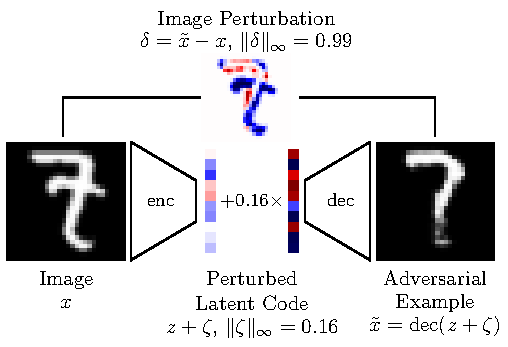
\includegraphics[width=1\textwidth]{main_illustration_c.pdf}
    \end{subfigure}
    \begin{subfigure}{0.18\textwidth}
        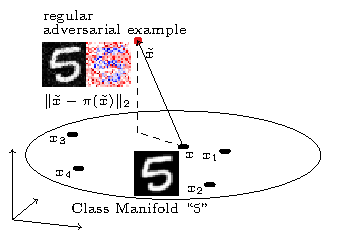
\includegraphics[width=1\textwidth,trim={0 0 1.9cm 0},clip]{main_illustration_a.pdf}
    \end{subfigure}
    \vskip -8px
    \caption{\red{Left: On-manifold adversarial examples can be computed using learned, class-specific \VAEGANs \cite{LarsenICML2016,RoscaARXIV2017}. The perturbation $\zeta$ is obtained via \eqnref{eq:main-on-manifold-attack} and added to the latent code $z = \enc(x)$ yielding the adversarial example $\tilde{x} = \dec(z + \zeta)$ with difference $\delta = \tilde{x} - x$ in image space. Right: The distance of a regular adversarial example $\tilde{x}$ to the manifold, approximated using nearest neighbors, is computed as the distance to its orthogonal projection $\pi(\tilde{x})$: $\|\tilde{x} - \pi(\tilde{x})\|_2$. Large distances indicate that the adversarial example likely left the manifold.}}
    \label{fig:main-illustration-2}
    \vskip 0px
\end{figure}

\vskip 0px
\subsection{On-Manifold Robustness is Essentially\\[2px]\hspace*{-5px}Generalization}

\begin{figure*}
    \centering
    \vskip -0.3cm
    \hskip -0.25cm
    \begin{subfigure}[t]{0.24\textwidth}
        \vskip 0px
        \centering
        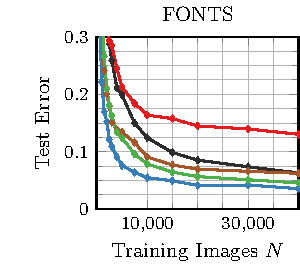
\includegraphics[width=1\textwidth]{experiments_hypo3_fonts_error.pdf}
    \end{subfigure}
    \begin{subfigure}[t]{0.24\textwidth}
        \vskip 0px
        \centering
        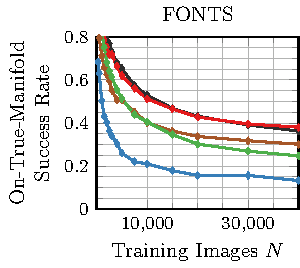
\includegraphics[width=1\textwidth]{experiments_hypo3_fonts_on_true.pdf}
    \end{subfigure}
    \begin{subfigure}[t]{0.24\textwidth}
        \vskip 0px
        \centering
        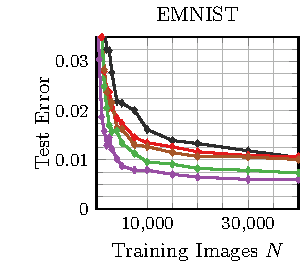
\includegraphics[width=1\textwidth]{experiments_hypo3_emnist_error.pdf}
    \end{subfigure}
    \begin{subfigure}[t]{0.24\textwidth}
        \vskip 0px
        \centering
        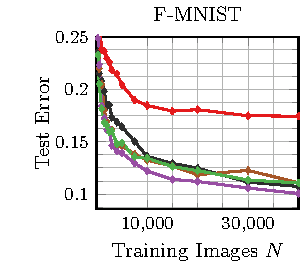
\includegraphics[width=1\textwidth]{experiments_hypo3_fashion_error.pdf}
    \end{subfigure}
    \\
    \hskip -0.25cm
    \begin{subfigure}[t]{0.24\textwidth}
        \vskip 0px
        \centering
        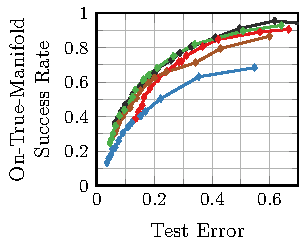
\includegraphics[width=1\textwidth]{experiments_hypo3_fonts_error_on_true_alt.pdf}
    \end{subfigure}
    \begin{subfigure}[t]{0.24\textwidth}
        \vskip 0px
        \centering
        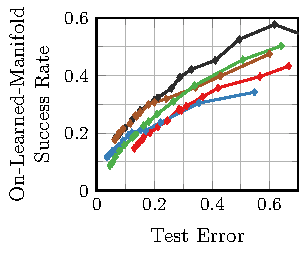
\includegraphics[width=1\textwidth]{experiments_hypo3_fonts_error_on_learned_alt.pdf}
    \end{subfigure}
    \begin{subfigure}[t]{0.24\textwidth}
        \vskip 0px
        \centering
        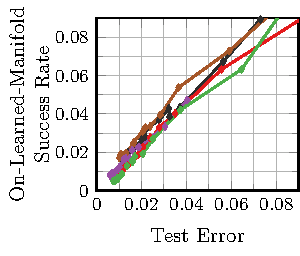
\includegraphics[width=1\textwidth]{experiments_hypo3_emnist_error_on_learned_alt.pdf}
    \end{subfigure}
    \begin{subfigure}[t]{0.24\textwidth}
        \vskip 0px
        \centering
        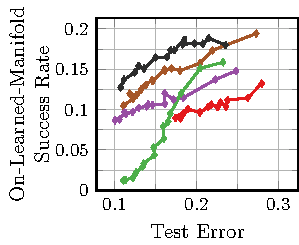
\includegraphics[width=1\textwidth]{experiments_hypo3_fashion_error_on_learned_alt.pdf}
    \end{subfigure}
    \\
    \fcolorbox{black!50}{white}{
    \begin{subfigure}[t]{0.975\textwidth}
        \centering
        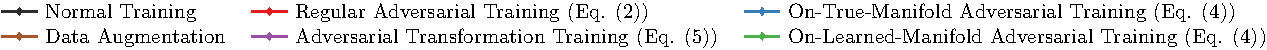
\includegraphics[width=0.9\textwidth]{experiments_hypo3_legend.pdf}
    \end{subfigure}
    }
    \vskip -6px
    \caption{On-manifold robustness is strongly related to generalization, as shown on \Fonts, \MNIST and \Fashion considering on-manifold success rate and test error. Top: test error and on-manifold success rate in relation to the number of training images. As test error reduces, so does on-manifold success rate. Bottom: on-manifold success rate plotted against test error reveals the strong relationship between on-manifold robustness and generalization.}
    \label{fig:main-hypo3}
    \vskip 0px
\end{figure*}

We argue that on-manifold robustness is nothing different than generalization: as on-manifold adversarial examples have non-zero probability under the data distribution, they are merely generalization errors. This is shown in \figref{fig:main-hypo3} (top left) where test error and on-manifold success rate on \Fonts are shown. As expected, better generalization, \ie, using more training images $N$, also reduces on-manifold success rate. In order to make this relationship explicit, \figref{fig:main-hypo3} (bottom) plots on-manifold success rate against test error. Then, especially for \Fonts and \MNIST, the relationship of on-manifold robustness and generalization becomes apparent. On \Fashion, the relationship is less pronounced because on-manifold adversarial examples, computed using our \VAEGANs, are not close enough to real generalization errors. However, even on \Fashion, the experiments show a clear relationship between on-manifold robustness and generalization.

\vskip 0px
\subsubsection{On-Manifold Adversarial Training\\[2px]Boosts Generalization}

Given that generalization positively influences on-manifold robustness, we propose to adapt adversarial training to the on-manifold case in order to boost generalization:
\vskip -14px
\begin{align}
    \min_w \sum_{n=1}^N \max_{\|\zeta\|_{\infty} \leq \eta} \cL(f(\dec(z_n + \zeta); w), y_n).
    \label{eq:main-on-manifold-adversarial-training}
\end{align}
\vskip -2px
\noindent with $z_n = \dec(x_n)$ being the latent codes corresponding to training images $x_n$. Then, on-manifold adversarial training corresponds to robust optimization \wrt the true, or approximated, data distribution. For example, with \matthias{the} perfect decoder on \Fonts, the inner optimization problem finds ``hard'' images irrespective of their likelihood under the data distribution. For approximate $\dec$, the benefit of on-manifold adversarial training depends on how well the true data distribution is matched, \ie, how realistic the obtained on-manifold adversarial examples are; in our case, this depends on the quality of the learned \VAEGANs.

\begin{figure*}
    \centering
    \vskip -0.3cm
    \hskip -0.25cm
    \begin{subfigure}[t]{0.24\textwidth}
        \vskip 0px
        \centering
        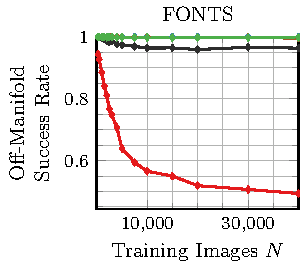
\includegraphics[width=1\textwidth]{experiments_hypo4_fonts_off.pdf}
    \end{subfigure}
    \begin{subfigure}[t]{0.24\textwidth}
        \vskip 0px
        \centering
        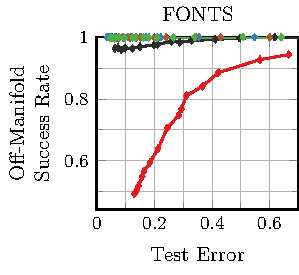
\includegraphics[width=1\textwidth]{experiments_hypo4_fonts_error_off_alt.pdf}
    \end{subfigure}
    \begin{subfigure}[t]{0.24\textwidth}
        \vskip 0px
        \centering
        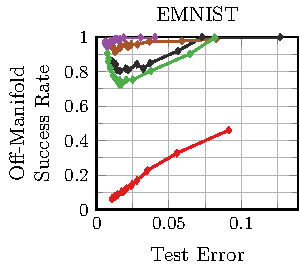
\includegraphics[width=1\textwidth]{experiments_hypo4_emnist_error_off_alt.pdf}
    \end{subfigure}
    \begin{subfigure}[t]{0.24\textwidth}
        \vskip 0px
        \centering
        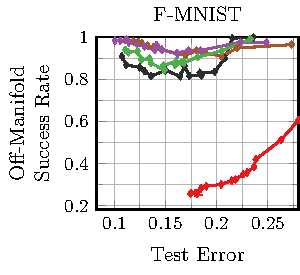
\includegraphics[width=1\textwidth]{experiments_hypo4_fashion_error_off_alt.pdf}
    \end{subfigure}
    \\
    \fcolorbox{black!50}{white}{
    \begin{subfigure}[t]{0.975\textwidth}
        \centering
        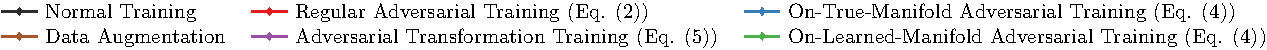
\includegraphics[width=0.9\textwidth]{experiments_hypo4_legend.pdf}
    \end{subfigure}
    }
    \vskip -6px
    \caption{Regular robustness is not related to generalization, as demonstrated on \Fonts, \MNIST and \Fashion considering test error and (regular) success rate. On \Fonts (left), success rate is not influenced by test error, except for adversarial training. Plotting success rate against test error highlights the independence of robustness and generalization; however, different training strategies exhibit different robustness-generalization characteristics.}
    \label{fig:main-hypo4}
    \vskip 0px
\end{figure*}

Instead of approximating the manifold using generative models, we can exploit known invariances of the data. Then, adversarial training can be applied to these invariances, assuming that they are part of the true manifold. In practice, this can, for example, be accomplished using adversarial deformations \cite{AlaifariARXIV2018,XiaoICLR2018,EngstromARXIV2017}, \ie, adversarially crafted transformations of the image. For example, as on \Fonts, we consider $6$-degrees-of-freedom transformations corresponding to translation, shear, scaling and rotation:
\vskip -14px
\begin{align}
    \min_w \sum_{n = 1}^N \max_{\|t\|_{\infty} \leq \eta, t \in \mR^6} \cL(f(T(x_n; t); w), y_n).
    \label{eq:main-stn-adversarial-training}
\end{align}
\vskip -2px
\noindent where $T(x; t)$ denotes the transformation of image $x$ with parameters $t$ and the $\eta$-constraint ensures similarity and label invariance. Again, the transformations can be applied using spatial transformer networks \cite{JaderbergNIPS2015} such that $T$ is differentiable; $t$ can additionally be constrained to a reasonable space of transformations. We note that a similar approach has been used by Fawzi \etal \cite{FawziICIP2016} to boost generalization on, \eg, MNIST \cite{LecunIEEE1998}. However, the approach was considered as an adversarial variant of data augmentation and not motivated through the lens of on-manifold robustness. We refer to \eqnref{eq:main-stn-adversarial-training} as adversarial transformation training and note that, on \Fonts, this approach is equivalent to on-manifold adversarial training as the transformations coincide with the actual, true manifold by construction. We also include a data augmentation baseline, where the transformations $t$ are applied randomly.

We demonstrate the effectiveness of on-manifold adversarial training in \figref{fig:main-hypo3} (top). On \Fonts, with access to the true manifold, on-manifold adversarial training is able to boost generalization significantly, especially for low $N$, \ie, few training images. Our \VAEGAN approximation on \Fonts seems to be good enough to preserve the benefit of on-manifold adversarial training. On \MNIST and \Fashion, the benefit reduces with the difficulty of approximating the manifold; this is the ``cost'' of imperfect approximation. While the benefit is still significant on \MNIST, it diminishes on \Fashion. However, both on \MNIST and \Fashion, identifying invariances and utilizing adversarial transformation training recovers the boost in generalization; especially in contrast to the random data augmentation baseline. Overall, on-manifold adversarial training is a promising tool for improving generalization and we expect its benefit to increase with better generative models.

\vskip 0px
\subsection{Regular Robustness is Independent of\\[2px]\hspace*{-5px}Generalization}

\red{We argue that generalization, as measured \emph{on} the manifold \wrt the data distribution, is mostly independent of robustness against regular, possibly off-manifold, adversarial examples when varying the amount of training data}. Specifically, in \figref{fig:main-hypo4} (left) for \Fonts, it can be observed that -- except for adversarial training -- the success rate is invariant to the test error. \red{This can best be seen when plotting the success rate against test error for different numbers of training examples, \cf \figref{fig:main-hypo4} (middle left): only for adversarial training there exists a clear relationship; for the remaining training schemes success rate is barely influenced by the test error. In particular, better generalization does not worsen robustness.} Similar behavior can be observed on \MNIST and \Fashion, see \figref{fig:main-hypo4} (right). Here, it can also be seen that different training strategies exhibit different characteristics \wrt robustness and generalization. \red{Overall, regular robustness and generalization are not necessarily contradicting goals.}

As mentioned in \secref{sec:introduction}, these findings are in contrast to related work \cite{TsiprasARXIV2018,SuARXV2018} claiming that an inherent trade-off between robustness and generalization exists. For example, Tsipras \etal \cite{TsiprasARXIV2018} use a synthetic toy dataset to theoretically show that no model can be both robust and accurate (on this dataset). However, they allow the adversary to produce perturbations that change the actual, true label \wrt the data distribution, \ie, the considered adversarial examples are not adversarial examples according to \defref{def:main-on-manifold-adversarial-example}. Thus, it is unclear whether the suggested trade-off actually exists \red{for real datasets}; our experiments, \red{at least, as well as further analysis in the supplementary material} seem to indicate the contrary. Similarly, Su \etal \cite{SuARXV2018} experimentally show a trade-off between adversarial robustness and generalization by studying different models on ImageNet \cite{RussakovskyIJCV2015}. However, Su \etal compare the robustness and generalization characteristics of different models (\ie, different architectures, training strategies \etc), while we found that the generalization performance does not influence robustness for any \emph{arbitrary, but fixed} model.

\vskip 0px
\subsection{Discussion}
\label{subsec:main-discussion}

Our results imply that robustness and generalization are not \red{necessarily} conflicting goals, as believed in related work \cite{TsiprasARXIV2018,SuARXV2018}. This means, in practice, for any arbitrary but fixed model, better generalization will not worsen regular robustness. Different models (architectures, training strategies \etc) might, however, exhibit different robustness and generalization characteristics, as also shown in \cite{SuARXV2018,RozsaICMLA2016}. For adversarial training, on regular adversarial examples, the commonly observed trade-off between robustness and generalization is explained by the tendency of adversarial examples to leave the manifold. As result, the network has to learn (seemingly) random, but adversarial, noise patterns \emph{in addition} to the actual task at hand; rendering the learning problem harder. On simple datasets, such as \MNIST, these adversarial directions might avoid overfitting; on harder tasks, \eg, \Fonts or \Fashion, the discrepancy in test error between normal and adversarial training increases. \red{Our results also support the hypothesis that regular adversarial training has higher sample complexity \cite{SchmidtARXIV2018,KhouryARXIV2018}. In fact, on \Fonts, adversarial training can reach the same accuracy as normal training with roughly twice the amount of training data, as demonstrated in \figref{fig:main-disc-2} (top). Furthermore, as illustrated in \figref{fig:main-disc-2} (bottom), the trade-off between regular robustness and generalization can be controlled by combining regular and on-manifold adversarial training, \ie boost generalization while reducing robustness.}

\begin{figure}
    \centering
    \vskip -0.3cm
    \hskip -0.25cm
    \begin{subfigure}[t]{0.235\textwidth}
        \vskip 0px
        \centering
        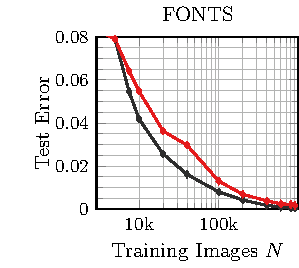
\includegraphics[width=1\textwidth]{experiments_disc_fonts_error_resnet.pdf}
    \end{subfigure}
    \begin{subfigure}[t]{0.235\textwidth}
        \vskip 0px
        \centering
        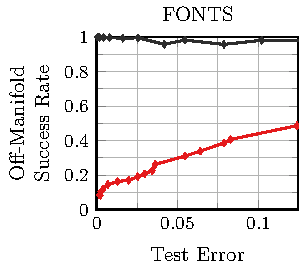
\includegraphics[width=1\textwidth]{experiments_disc_fonts_error_off_resnet.pdf}
    \end{subfigure}
    \\
    \begin{subfigure}[t]{0.235\textwidth}
        \vskip 0px
        \centering
        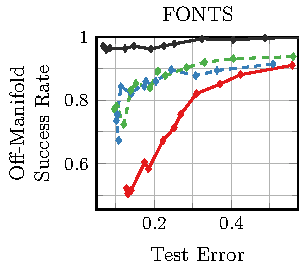
\includegraphics[width=1\textwidth]{experiments_disc_fonts_error_off_accuracy.pdf}
    \end{subfigure}
    \begin{subfigure}[t]{0.235\textwidth}
        \vskip 0px
        \centering
        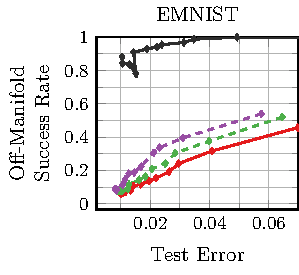
\includegraphics[width=1\textwidth]{experiments_disc_emnist_error_off_accuracy.pdf}
    \end{subfigure}
    \\[-2px]
    \fcolorbox{black!50}{white}{
    \begin{subfigure}[t]{0.45\textwidth}
        \centering
        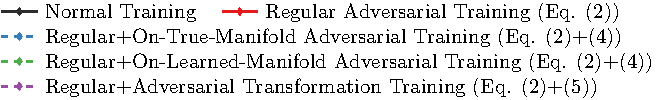
\includegraphics[width=1.025\textwidth]{experiments_disc_2_legend.pdf}
    \end{subfigure}
    }
    \vskip -6px
    \caption{\red{Adversarial training on regular adversarial examples, potentially leaving the manifold, renders the learning problem more difficult. Top: With roughly $1.5$ to $2$ times the training data, adversarial training can still reach the same accuracy as normal training; results for ResNet-13~\cite{HeCVPR2016}. Bottom: Additionally, the trade-off can be controlled by combining regular and on-manifold adversarial training; results averaged over $3$ models.}}
    \label{fig:main-disc-2}
    \vskip 0px
\end{figure}

The presented results can also be confirmed on more complex datasets, such as \Celeb, and using different threat models, \ie, attacks. On \Celeb, where \VAEGANs have difficulties approximating the manifold, \figref{fig:main-disc-1} (top left) shows that on-manifold robustness still improves with generalization although most on-manifold adversarial examples are not very realistic, see \figref{fig:main-examples}. Similarly, regular robustness, see \figref{fig:main-disc-1} (top right), is not influenced by generalization; here, we also show that the average distance of the perturbation, \ie, average $\|\delta\|_{\infty}$, when used to asses robustness leads to the same conclusions. Similarly, as shown in \figref{fig:main-disc-1} (bottom), our findings are confirmed using Carlini and Wagner's attack \cite{CarliniSP2017} with $L_2$-norm -- to show that the results generalize across norms. However, overall, we observed lower success rates using \cite{CarliniSP2017} and the $L_2$ norm. \red{Finally, our results can also be reproduced using transfer attacks (\ie, black-box attacks, which are generally assumed to be subsumed by white-box attacks \cite{AthalyeARXIV2018}) as well as and different architectures such as multi-layer perceptrons, ResNets~\cite{HeCVPR2016} and VGG~\cite{SimonyanARXIV2014}, as detailed in the supplementary material.}

\begin{figure}
    \centering
    \vskip -0.3cm
    \hskip -0.25cm
    \begin{subfigure}[t]{0.235\textwidth}
        \vskip 0px
        \centering
        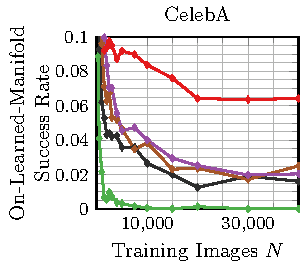
\includegraphics[width=1\textwidth]{experiments_disc_celeba_on_learned.pdf}
    \end{subfigure}
    \begin{subfigure}[t]{0.235\textwidth}
        \vskip 0px
        \centering
        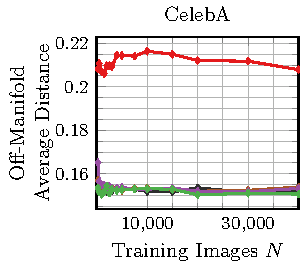
\includegraphics[width=1\textwidth]{experiments_disc_celeba_off_distance.pdf}
    \end{subfigure}
    \\
    \hskip -0.25cm
    \begin{subfigure}[t]{0.235\textwidth}
        \vskip 0px
        \centering
        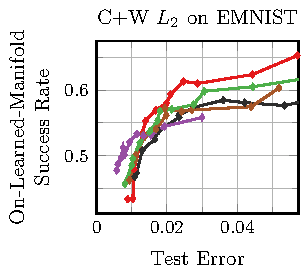
\includegraphics[width=1\textwidth]{experiments_disc_emnist_error_on_learned_cw_alt.pdf}
    \end{subfigure}
    \begin{subfigure}[t]{0.235\textwidth}
        \vskip 0px
        \centering
        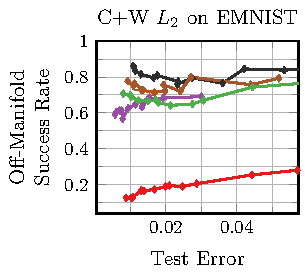
\includegraphics[width=1\textwidth]{experiments_disc_emnist_error_off_cw_alt.pdf}
    \end{subfigure}
    \\[-2px]
    \fcolorbox{black!50}{white}{
    \begin{subfigure}[t]{0.45\textwidth}
        \centering
        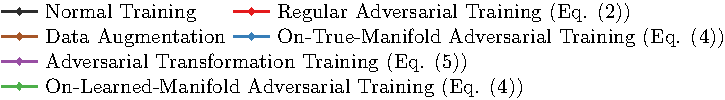
\includegraphics[width=1.01\textwidth]{experiments_disc_1_legend.pdf}
    \end{subfigure}
    }
    \vskip -6px
    \caption{Results on \Celeb and using the $L_2$ Carlini and Wagner \cite{CarliniSP2017} attack. On \Celeb, as the class manifolds are significantly harder to approximate, the benefit of on-manifold adversarial training diminishes. For \cite{CarliniSP2017}, we used $120$ iterations; our hypotheses are confirmed, although \cite{CarliniSP2017} does not use the training loss as attack objective and the $L_2$ norm changes the similarity-constraint for regular and on-manifold adversarial examples.}
    \label{fig:main-disc-1}
    \vskip 0px
\end{figure}